
\subsection{Innlogging}
\begin{itemize}
  \item Brukeren skirver inn brukernavn og passord.
  \item Dersom brukeren har skrevet inn riktig brukernavn og passord når han trykker på logg inn vil han bli sendt videre til kalendersystemet.
  \item Dersom brukeren har skrevet feil eller ugyldig informasjon i et av feltene vil han få en feilmelding.
\end{itemize}

\subsection{Lage avtale}
\begin{itemize}
  \item Brukeren skriver inn tittel på avtale/møte, denne kan han definere selv. 
\item Tekstfeltene Start, slutt, og alarm blir satt ved å trykke på “Åpne kalender”-knappen. Da vil et pop-up vindu åpne seg, hvor du kan trykke på hvilken dato du vil velge via en kalender, og skrive inn tidspunkt. Start, slutt og Alarm feltene er det bare mulig å endre på via “Åpne kalender”-knappen.
 \item Beskrivelse er et åpent felt hvor du kan skrive hva du vil.
Combobox ved Kalender vil la deg velge hvilken av dine kalendere du vil at avtalen skal lagres. 
\item Under deltagere har du en tom liste, og to ved siden av. 
\item Du kan legge til deltagere ved å trykke på pluss-tegnet, fordi da vil AddParticipantPanel åpne seg.
\item Hvis du selecter en person som finnes i listen og trykker på minus-tegnet vil den personen bli fjernet fra listen. 
\item Tilbake-knappen vil føre deg tilbake til CalendarLayout, Lagre vil føre deg videre til SavedMeetingPanel, og slett vil naturligvis føre deg tilbake til CalendarLayout.
\end{itemize}

\subsection{Avtalevisning}
\begin{itemize}
\item Her ser man oversikten over møte.
\item Feltene i dette vinduet kan ikke redigeres.
\item Dersom man trykker på godta vil man bli lagt til i listen kommer og godta-knappen vil bli grået ut.
\item Dersom man trykker på avslå vil man bli lagt til i listen over kommer ikke og avslå-knappen vil bli grået ut.
\item Dersom man er møteleder vil man også se knappene Send ut møteinnkalling og Rediger, inviterte brukere vil ikke se disse knappene.
\item Dersom en møteinnkalling er send ut vil send ut møteinnkalling-knappen forsvinne.
\end{itemize}

\subsection{Kalendervisning}
\begin{itemize}
\item I kalendertabellen vil møtene og avtalene man skal på bli lagt inn.
\item Avtalene og møtene vil bli lagt inn i cellen som passer til tidspunktet hendelsen skal foregå.
\item Dersom man har flere avtaler på samme tidspunkt vil disse dele plassen i ruten.
\item Om man trykker på en avtale eller et møte vil man komme inn på møte.
\item Dersom man trykker på legg til avtale vil man bli sendt videre til siden hvor man kan lage en avtale eller et møte.
\item Under Notifikasjoner vil man få en liste over alle notifikasjonene man har, disse kan man klikke seg inn på for å bli sendt videre til gjeldene avtale.
\item I tekstfeltet under Mine kalendere kan man skrive inn navn på en ny kalender, og trykke på knappen ved siden av tekstfeltet for å få opp et nytt vindu, som gir deg forskjellige valgmuligheter vedrørende din nye kalender.
\item Dersom man dobbelklikker på en av kalenderene i listen over sine kalendere eller andre kalendere blir man sendt til et vindu med mer informasjon om kalenderen.
\item Over kalenderen vises hvilke uke man ser på, og man kan bla gjennom de ulike bildene ved knappene på sidene.
\item Dersom man klikker på logg ut, vil brukeren bli logget ut og sendt til innloggingsvinduet igjen.
\end{itemize}

\subsection{legge til deltager}
\begin{itemize}
\item Her er panelet der man kan legge til flere deltagere til et møte.
\item Under brukernavn og gruppe, er det en dropdown-liste som viser listen over alle brukerne.
\item Her vil alle deltageren som er valgt legges til i avtalen.
\item Det droppes ned ei liste med deltager, man kan trykke på dem for å velge og trykke legg til for å legge til personen.
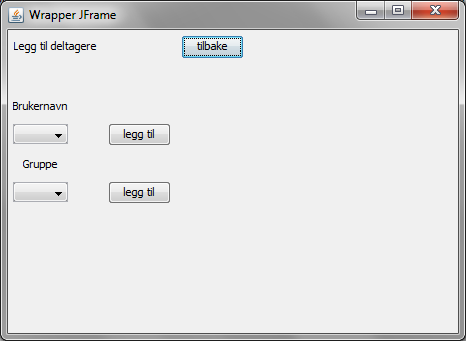
\includegraphics[scale=0.5]{AddPersonPanel.png}
\item Man kan velge slik at det dropper ned ei liste med forskjellige grupper, man kan trykke på den for å markere dem og legge til grupper på samme måte som brukere.
\item Når man legger til en bruker vil systemet gå gjennom alle brukerne i gruppen og legge dem til i møte.
\item Til høyre har vi ei liste som viser alle deltagerne som er valgt.
\end{itemize}


\subsection{har kan man bestille møtelokale}
\begin{itemize}
\item Her får man lagt til et møtelokale.
\item Vi har her et tekstfelt som lar brukeren velge hvor mange personer rommet skal kunne ha plass til. 
\item Under er det et view over start og slutt tidspunktet på avtalen. 
\item Nederst er det en liste med rom som passer til kriterier om hvor mange det skal være plass til og som ikke er opptatt i gjeldene tidsrom.
\item Når man trykker på et av rommene, så vil det rommet bli merkert.
\item Så trykker man “velg rom” for å legge til rommet som møtelokalet.
\end{itemize}

\subsection{ManageCalendarsJDialog:}
\begin{itemize}
\item Her har man forskjellige valgmuligheter for kalenderen man har valgt. \item Først er det en drop-down-menu hvor man kan velge hvilken farge kalenderen skal ha.
\item Det er også en checkbox, hvor du bestemmer om kalenderen skal være synlig på hovedkalenderen din eller ikke. 
\item Nederst er det to knapper for avbryt og lagre. 
\end{itemize}
